\documentclass[10pt,graphicx,caption,rotating]{article}
\textheight=25cm
\textwidth=18cm
\topmargin=-2cm
\oddsidemargin=0cm
\usepackage[utf8x]{inputenc}
\usepackage{graphicx}
\usepackage{times}
\usepackage[tbtags]{amsmath}
\usepackage{cite}
\usepackage[all]{xy}
\usepackage{subfigure}
\usepackage{wrapfig}
\usepackage{multicol}
\usepackage{url}
\usepackage[tbtags]{amsmath}
\usepackage{amsmath,amssymb,amsfonts,amsbsy}
\usepackage{bm}
\usepackage[all]{xy}
\usepackage[centerlast, small]{caption}
\usepackage[colorlinks=true, citecolor=blue, linkcolor=blue, urlcolor=blue, breaklinks=true]{hyperref}

\begin{document}

\begin{figure}[h]
    \begin{minipage}[t]{1cm}
    \centering
        \subfigure[Se\~nal Original Punto A]{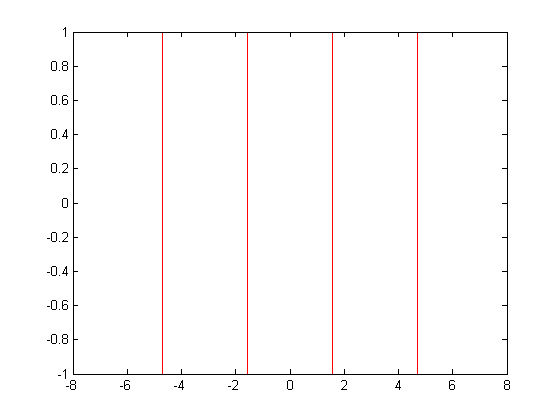
\includegraphics[scale=0.6]{1.png}}
    \end{minipage}
    \hfill\begin{minipage}[t]{10cm}
    \centering
        \subfigure[Funci\'on con 1 coeficiente]{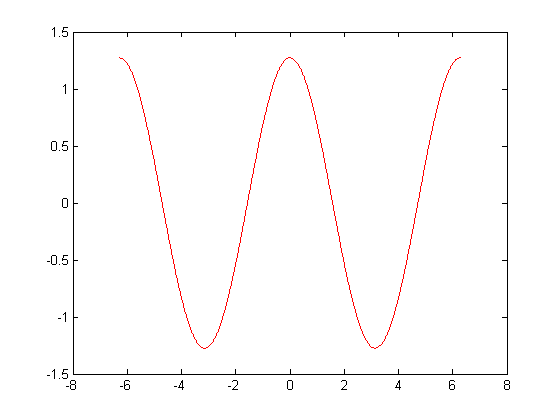
\includegraphics[scale=0.6]{2.png}}
    \end{minipage}\\
    \begin{minipage}[t]{1cm}
    \centering
        \subfigure[Funci\'on con 2 coeficientes]{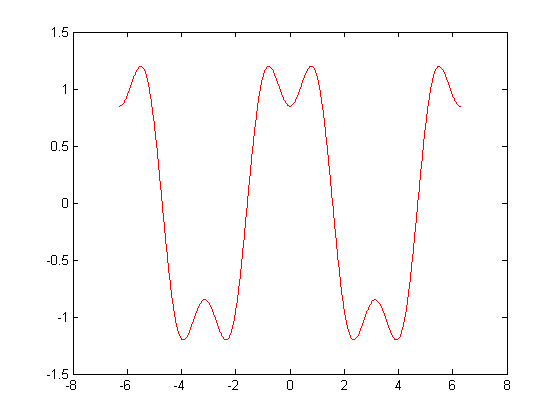
\includegraphics[scale=0.6]{3.png}}
    \end{minipage}
    \hfill\begin{minipage}[t]{10cm}
    \centering
        \subfigure[Funci\'on con 3 coeficientes]{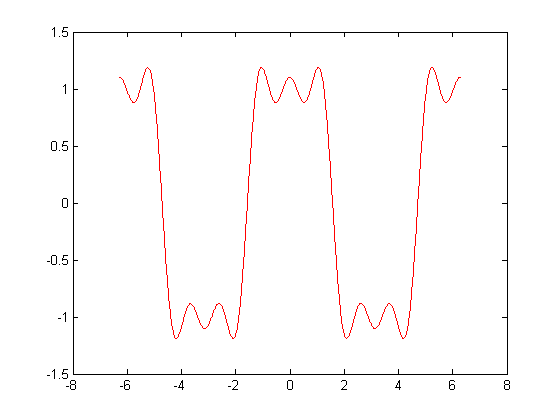
\includegraphics[scale=0.6]{4.png}}
    \end{minipage}\\
    \begin{minipage}[t]{1cm}
    \centering
        \subfigure[Se\~nal Original Punto B]{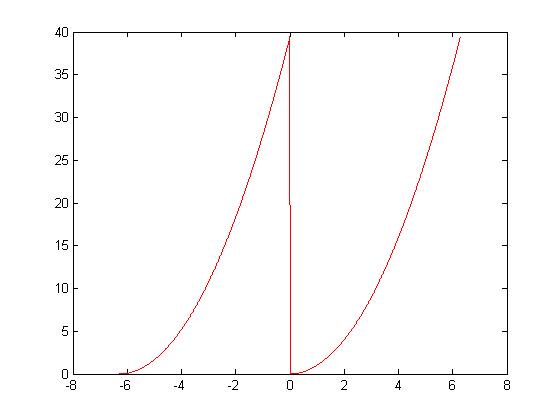
\includegraphics[scale=0.6]{5.png}}
    \end{minipage}
    \hfill\begin{minipage}[t]{10cm}
    \centering
        \subfigure[Funci\'on con 1 coeficiente]{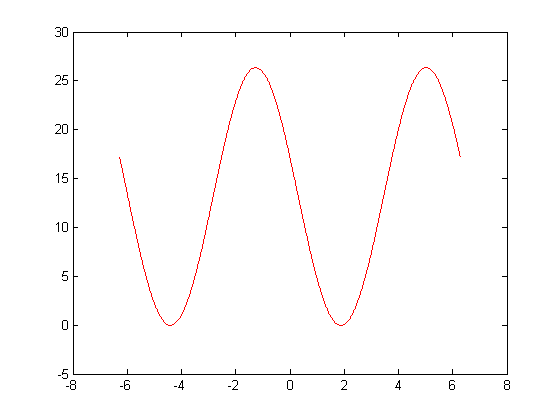
\includegraphics[scale=0.6]{6.png}}
    \end{minipage}
\end{figure}    

\begin{figure}[h]
    \begin{minipage}[t]{1cm}
    \centering
        \subfigure[Funci\'on con 2 coeficientes]{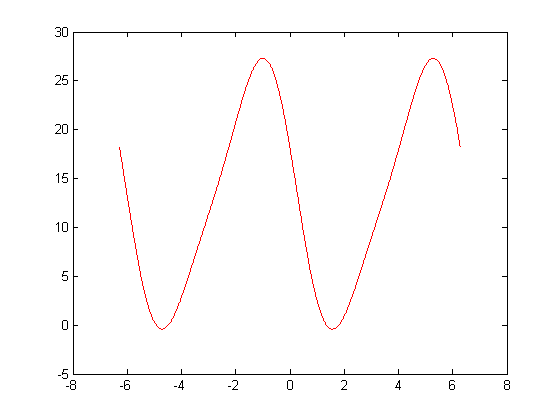
\includegraphics[scale=0.6]{7.png}}
    \end{minipage}
    \hfill\begin{minipage}[t]{10cm}
    \centering
        \subfigure[Funci\'on con 3 coeficientes]{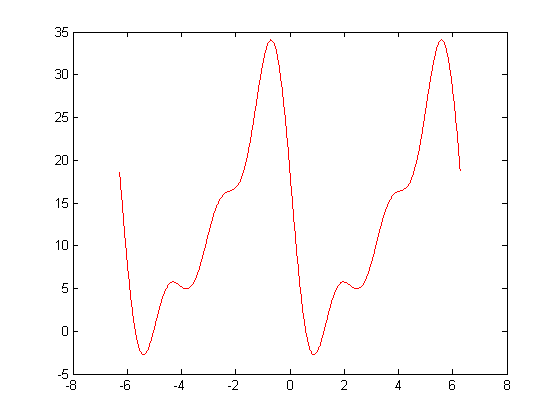
\includegraphics[scale=0.6]{8.png}}
    \end{minipage}\\
    \begin{minipage}[t]{1cm}
    \centering
        \subfigure[Se\~nal Original Punto C]{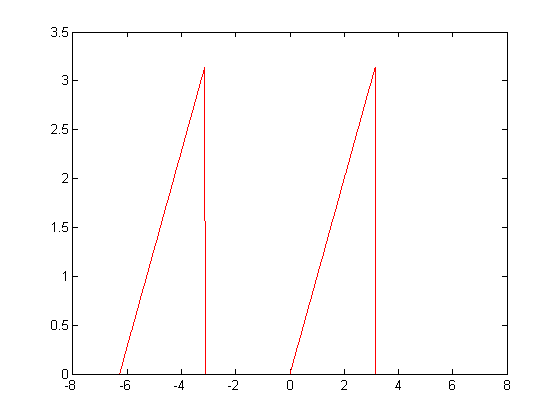
\includegraphics[scale=0.6]{9.png}}
    \end{minipage}
    \hfill\begin{minipage}[t]{10cm}
    \centering
        \subfigure[Funci\'on con 1 coeficiente]{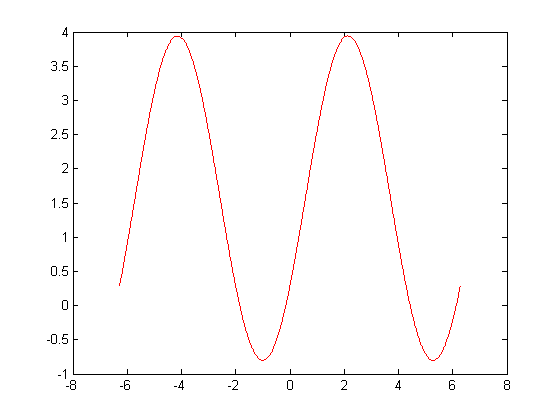
\includegraphics[scale=0.6]{10.png}}
    \end{minipage}\\
    \begin{minipage}[t]{1cm}
    \centering
        \subfigure[Funci\'on con 2 coeficientes]{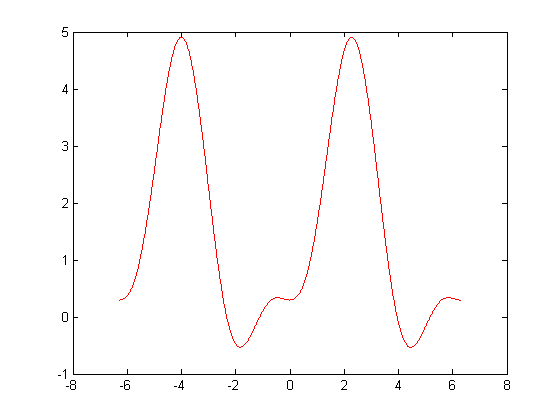
\includegraphics[scale=0.6]{11.png}}
    \end{minipage}
    \hfill\begin{minipage}[t]{10cm}
    \centering
        \subfigure[Funci\'on con 3 coeficientes]{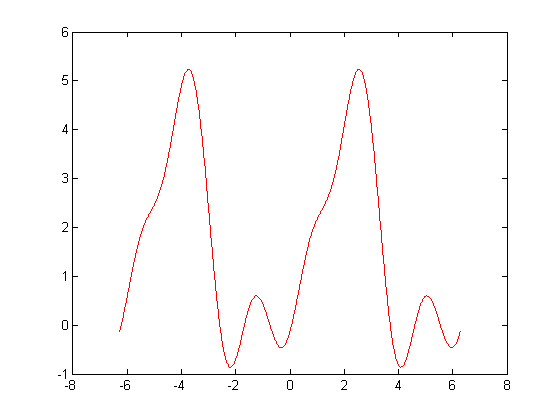
\includegraphics[scale=0.6]{12.png}}
    \end{minipage}
\end{figure}

\begin{figure}[h]
    \begin{minipage}[t]{1cm}
    \centering
        \subfigure[Se\~nal Original Punto C]{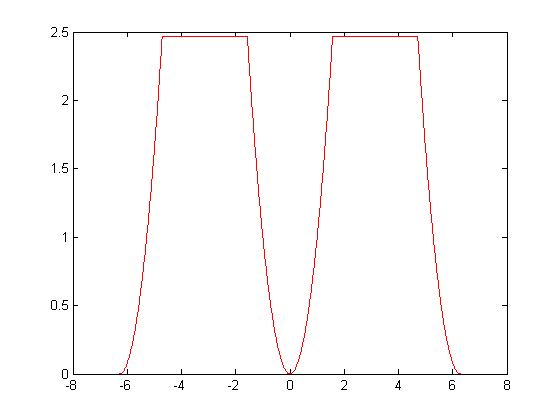
\includegraphics[scale=0.6]{13.png}}
    \end{minipage}
    \hfill\begin{minipage}[t]{10cm}
    \centering
        \subfigure[Funci\'on con 1 coeficiente]{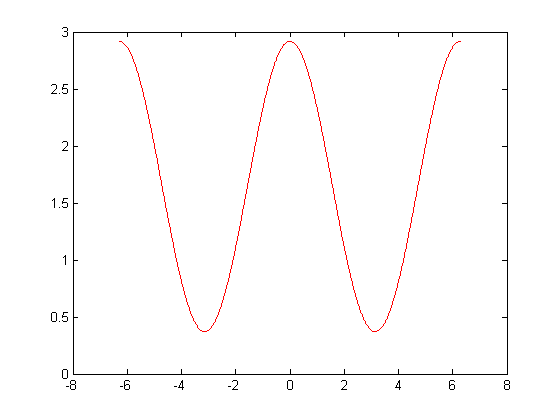
\includegraphics[scale=0.6]{14.png}}
    \end{minipage}\\
    \begin{minipage}[t]{1cm}
    \centering
        \subfigure[Funci\'on con 2 coeficientes]{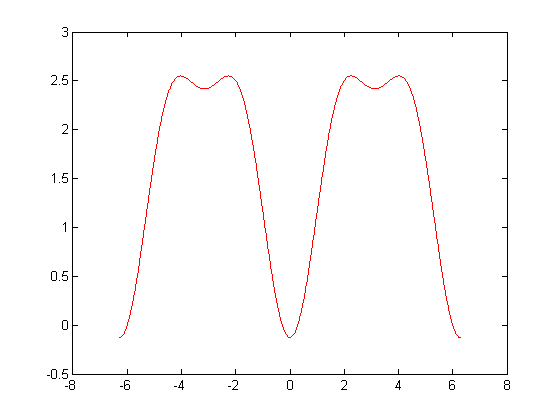
\includegraphics[scale=0.6]{15.png}}
    \end{minipage}
    \hfill\begin{minipage}[t]{10cm}
    \centering
        \subfigure[Funci\'on con 3 coeficientes]{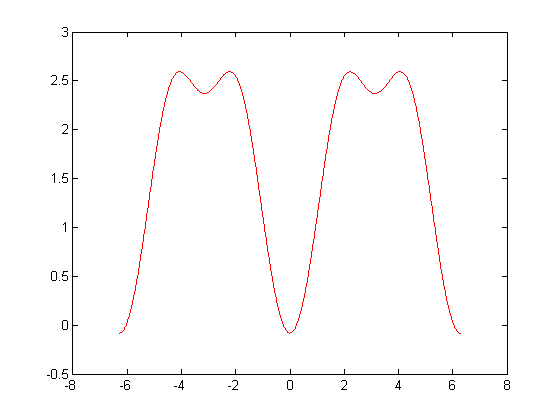
\includegraphics[scale=0.6]{16.png}}
    \end{minipage}
\end{figure}

\end{document} 